%Incidencia de una onda plana a 45° con n_i = 1, n_t = 1.46   

\documentclass[tikz,border=1cm]{standalone}
\usepackage{physics}
\usepackage{tikz}
\usetikzlibrary{decorations.pathreplacing,decorations.pathmorphing}

\begin{document}


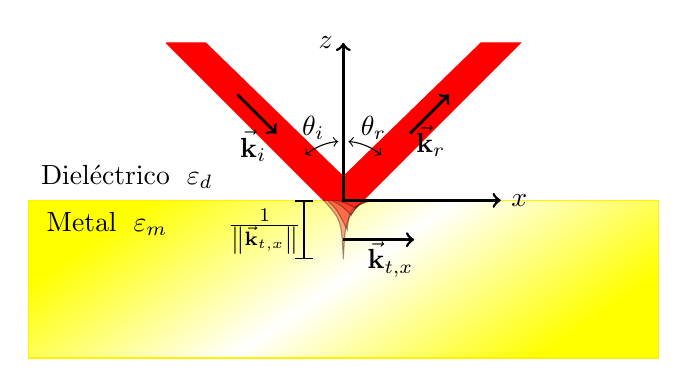
\begin{tikzpicture}%[   ESTO PONE LAS RAYAS QUE USO EN EPSEJOS
%    interface/.style={
        % The border decoration is a path replacing decorator. 
        % For the interface style we want to draw the original path.
        % The postaction option is therefore used to ensure that the
        % border decoration is drawn *after* the original path.
%        postaction={draw,decorate,decoration={border,angle=-45,
%                    amplitude=0.3cm,segment length=2mm}}},
%    ]



%-------------------------------------------- Incidence media
\shadedraw[	top color = yellow,				%%%%	Color de arriba
			bottom color =yellow,				%%%%	Color de abajo
			middle color = white, 			%%	Color de en medio
			shading angle = 35]			%%%%	Ángulo de gradiente
		 (-4,-2) rectangle (4,0);
% Interface
\draw[yellow,line width=.5pt](-4,0)--(4,0)--(4,-2)--(-4,-2)--(-4,0); %%..5pt, interface]
% Media names
\node at (-2.75,.3) {Diel\'ectrico $\; \varepsilon_d$}; 
\node at (-3,-.3) {Metal  $\; \varepsilon_m$};

%-------------------------------------------- Laser beam outside
\draw[fill=red, opacity = 1,red](-2.25,2)--(-1.75,2)-- (0,.3)  %%% outside the metal
						--(1.75,2)--(2.25,2)
						--(.25,0)--(-.25,0)--(-2.25,2);																														
%--------------------------------------------  Incident Wave
\path (0,0)++(112.5:1cm)node{$\theta_i$};       % Angle
\draw[<->](95:.75cm)arc(95:130:.75cm);
 
    \draw[->,line width=1pt](135:1.9cm)--(135:1.2cm);    %Wave vector
    \path (0,0)++(141:1.1cm)node[left]{$\va{k}_i$};     %Wave vector label
    
%--------------------------------------------  Reflected Wave
\path (0,0)++(67.5:1cm)node{$\theta_r$};       % Angle
\draw[<->](85:.75cm)arc(85:50:.75cm);
 
    \draw[->,line width=1pt](45:1.2cm)--(45:1.9cm);    %Wave vector
    \path (0,0)++(43:1.1cm)node[right]{$\va{k}_r$};     %Wave vector label
  
%--------------------------------------------  Transmitted Wave & Skin depth
\draw[fill = red, opacity = .35] (-.25,0) ..controls (-.025,-.25) .. (0,-.75)
											..controls (.025,-.25) .. (.25,0);  %1st evanescent wave
\draw[fill = red, opacity = .35] (-.2,0) ..controls (-.075,-.125) .. (0.05,-.375)
											..controls (.075,-.125) .. (.3,0);  %2nd evanescent wave
\draw[fill = red, opacity = .35] (-.15,0) ..controls (-.025,-.0625) .. (0.1,-.1875)
											..controls (.175,-.0625) .. (.35,0);  %3rd evanescent wave
\draw[fill = red, opacity = .35] (-.1,0) ..controls (.025,-.03125) .. (0.15,-.09375)
											..controls (.225,-.03125) .. (.4,0);  %4th evanescent wave	

    \draw[->,line width=1pt](0,-.5)--(.9,-.5);    %Wave vector
    \node at (.6,-.75) {$\va{k}_{t,x}$};
    
    \draw[|-|,line width=.2mm,black] (-.5,.0)--(-.5,-.75);%
    \node at (-1,-.4) {$\frac{1}{\norm{\va{k}_{t,x}}}$};
%--------------------------------------------  Axes
\draw[<->, line width =1pt] (0,2)node[left]{$z$}--(0,0) -- (2,0)node[right]{$x$};




\end{tikzpicture}
\end{document}